\section{VGA-controller}

We learned early on that last years group had problems with their off-the-shelf
\ac{VGA}-controller being a major bottleneck, and was only able to squeeze out less
than one frame per second. Since one of our goals ({\sc FR1}, see Table
\ref{fig:func-req}) with this project was to hit a minimum frame rate of ten
frames per second, going down the same route with the same controller was
obviously off the table.

After having scoured the Internet for higher-performing \ac{VGA}-controllers in our
price-range without any luck, and after consulting with Jahre, we decided on
implementing our own \ac{VGA}-controller within the \ac{FPGA}.

\section{VGA controller}

We learned early on that last years' group had problems with their off-the-shelf
\ac{VGA} controller being a major bottleneck, and were only able to squeeze out
less than one frame per second. Since one of our goals (FR1, Table
\ref{fig:func-req}) with this project was to hit a minimum frame rate of ten
frames per second, using a similar approach would most likely leave us with a
machine unable to fulfill FR1.

After having scoured the Internet for higher performing \ac{VGA} controllers in our
price range without any luck, and after consulting with Jahre, we decided to
implement our own \ac{VGA} controller on the \ac{FPGA}.

\section{VGA controller}

We learned early on that last years' group had problems with their off-the-shelf
\ac{VGA} controller being a major bottleneck, and were only able to squeeze out
less than one frame per second. Since one of our goals (FR1, Table
\ref{fig:func-req}) with this project was to hit a minimum frame rate of ten
frames per second, using a similar approach would most likely leave us with a
machine unable to fulfill FR1.

After having scoured the Internet for higher performing \ac{VGA} controllers in our
price range without any luck, and after consulting with Jahre, we decided to
implement our own \ac{VGA} controller on the \ac{FPGA}.

\section{VGA controller}

We learned early on that last years' group had problems with their off-the-shelf
\ac{VGA} controller being a major bottleneck, and were only able to squeeze out
less than one frame per second. Since one of our goals (FR1, Table
\ref{fig:func-req}) with this project was to hit a minimum frame rate of ten
frames per second, using a similar approach would most likely leave us with a
machine unable to fulfill FR1.

After having scoured the Internet for higher performing \ac{VGA} controllers in our
price range without any luck, and after consulting with Jahre, we decided to
implement our own \ac{VGA} controller on the \ac{FPGA}.

\input{fig/fpga/vga}

\subsection{Design}
We recognized the importance of allowing the control core to dump pixels to the
\ac{VGA} controller at its own pace without having to meet certain timing criteria,
so a physical memory and hence a memory controller was needed. Since the \ac{FPGA}
is running on 50MHz \TODO {This is wrong, system runs on 25MHz} and the pixel clock should be running on approximately
25MHz, a fairly simple solution for dividing the memory between the control
core and the actual signal generator was found: The signal generator must be
able to read from memory at most every other cycle, so the remaining cycles are
all free for the control core to use. To simplify the design as much as
possible, the memory controller simply alternates every cycle between writing
what is asserted on the signals from the control core, and reading a pixel
for the signal generator.

The signal generator itself is pretty straightforward. It calculates
when to pulse the V-sync and H-sync signals for a given resolution, and outputs
a (8-bit greyscale) pixel fetched from the memory controller at the appropriate
time.

\subsection{Circuitry}
\input{fig/fpga/vga-circuit} 

When designing the circuit, we had to choose between a black box \ac{DAC} and
making our own. Preliminary research on the \ac{VGA}-protocol showed that for
our purposes and our fairly low requirements on quality, making the \ac{DAC}
with simple resistors in parallel would be sufficient. Each resistor doubles in
resistance for each step from the most significant bit to the least
significant. We thought this would be easier to prototype and debug. The
resulting circuit is shown in Figure \ref{fig:vga-circuit}. Since color was a
``nice-to-have'' in case we had time to spare and not at all a priority, we made
the decision to greatly simplify the design by making the switch from greyscale
to color a manual operation of moving a set of jumpers. This way we reduced both
pin usage on the \ac{FPGA} and the complexity of the circuit.


\subsection{Design}
We recognized the importance of allowing the control core to dump pixels to the
\ac{VGA} controller at its own pace without having to meet certain timing criteria,
so a physical memory and hence a memory controller was needed. Since the \ac{FPGA}
is running on 50MHz \TODO {This is wrong, system runs on 25MHz} and the pixel clock should be running on approximately
25MHz, a fairly simple solution for dividing the memory between the control
core and the actual signal generator was found: The signal generator must be
able to read from memory at most every other cycle, so the remaining cycles are
all free for the control core to use. To simplify the design as much as
possible, the memory controller simply alternates every cycle between writing
what is asserted on the signals from the control core, and reading a pixel
for the signal generator.

The signal generator itself is pretty straightforward. It calculates
when to pulse the V-sync and H-sync signals for a given resolution, and outputs
a (8-bit greyscale) pixel fetched from the memory controller at the appropriate
time.

\subsection{Circuitry}
\begin{figure}[h!]
\centering
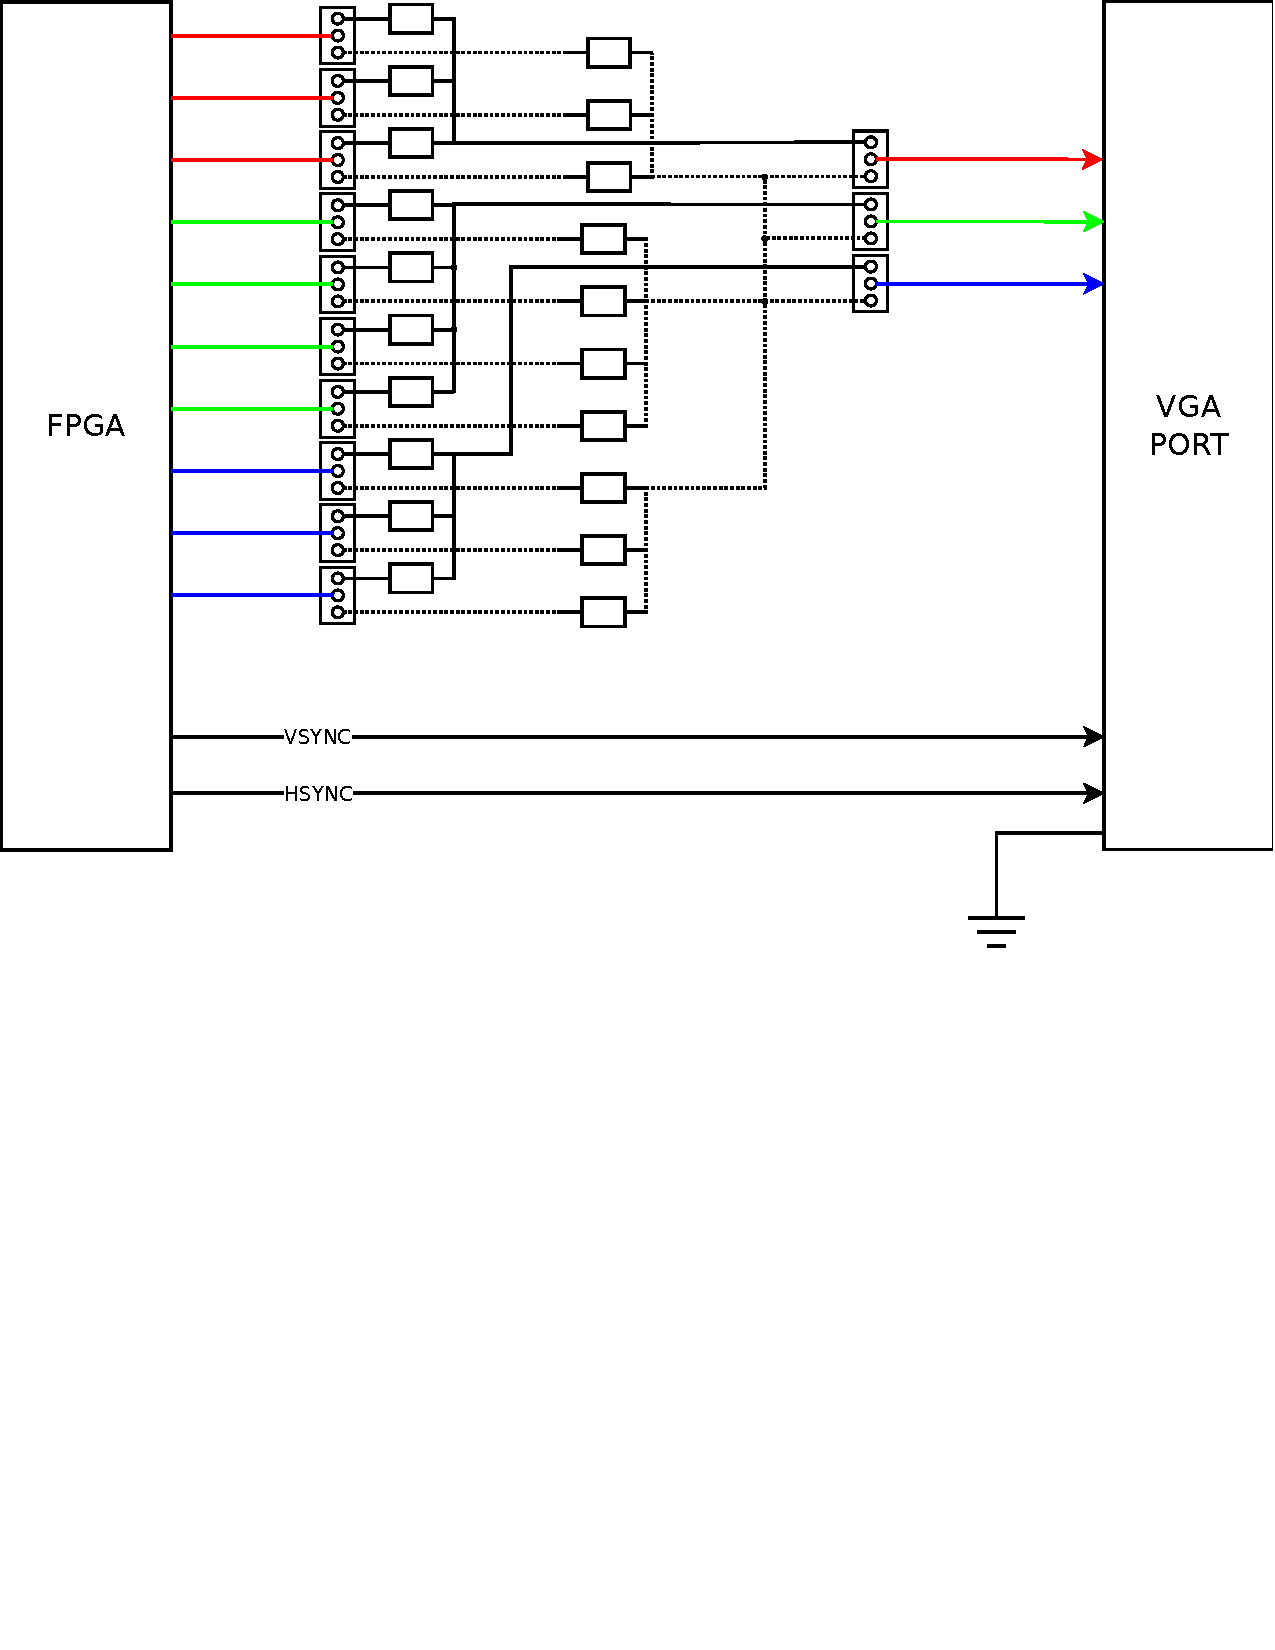
\includegraphics[width=\linewidth,clip,trim=0 11cm 0 0]
                {fig/fpga/vga-circuit.pdf}
\caption[VGA controller]
        {The resistor network of the DAC.}
\label{fig:vga-circuit}
\end{figure}
 

When designing the circuit, we had to choose between a black box \ac{DAC} and
making our own. Preliminary research on the \ac{VGA}-protocol showed that for
our purposes and our fairly low requirements on quality, making the \ac{DAC}
with simple resistors in parallel would be sufficient. Each resistor doubles in
resistance for each step from the most significant bit to the least
significant. We thought this would be easier to prototype and debug. The
resulting circuit is shown in Figure \ref{fig:vga-circuit}. Since color was a
``nice-to-have'' in case we had time to spare and not at all a priority, we made
the decision to greatly simplify the design by making the switch from greyscale
to color a manual operation of moving a set of jumpers. This way we reduced both
pin usage on the \ac{FPGA} and the complexity of the circuit.


\subsection{Design}
We recognized the importance of allowing the control core to dump pixels to the
\ac{VGA} controller at its own pace without having to meet certain timing criteria,
so a physical memory and hence a memory controller was needed. Since the \ac{FPGA}
is running on 50MHz \TODO {This is wrong, system runs on 25MHz} and the pixel clock should be running on approximately
25MHz, a fairly simple solution for dividing the memory between the control
core and the actual signal generator was found: The signal generator must be
able to read from memory at most every other cycle, so the remaining cycles are
all free for the control core to use. To simplify the design as much as
possible, the memory controller simply alternates every cycle between writing
what is asserted on the signals from the control core, and reading a pixel
for the signal generator.

The signal generator itself is pretty straightforward. It calculates
when to pulse the V-sync and H-sync signals for a given resolution, and outputs
a (8-bit greyscale) pixel fetched from the memory controller at the appropriate
time.

\subsection{Circuitry}
\begin{figure}[h!]
\centering
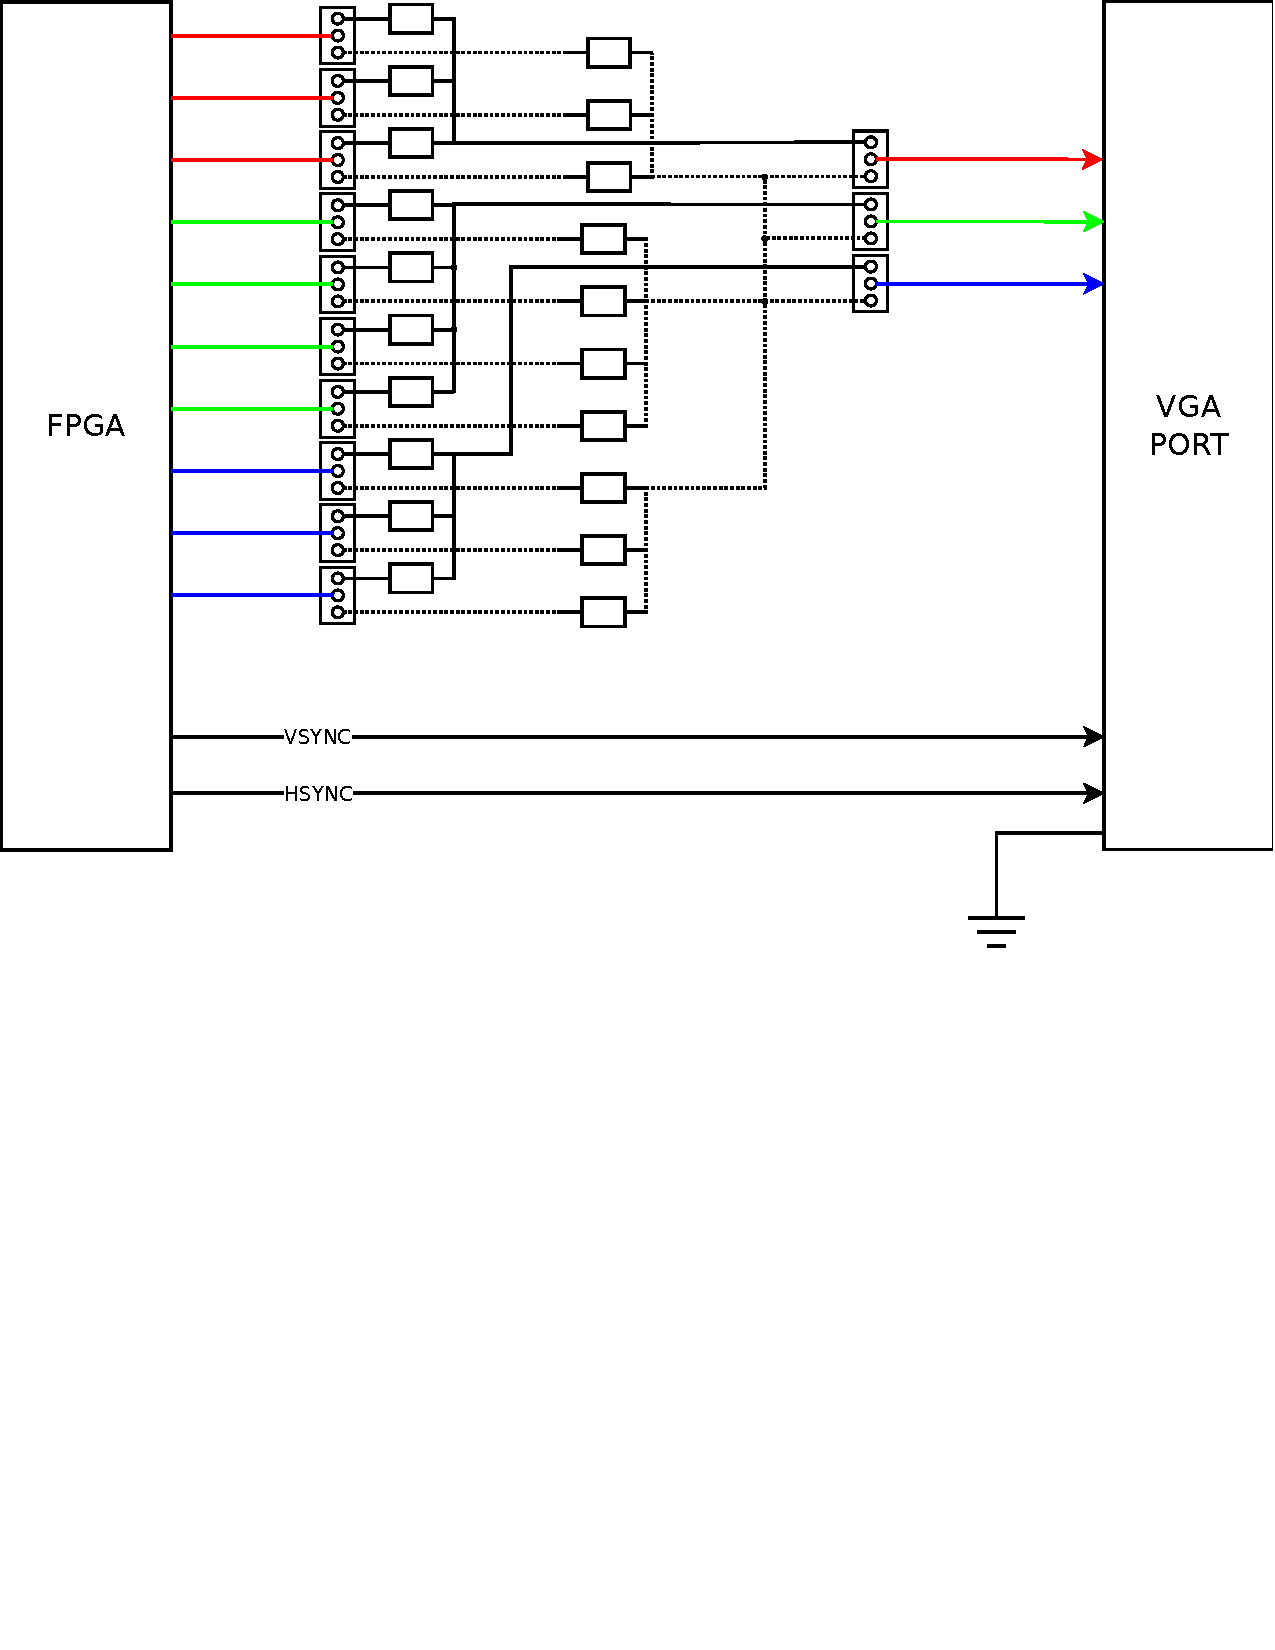
\includegraphics[width=\linewidth,clip,trim=0 11cm 0 0]
                {fig/fpga/vga-circuit.pdf}
\caption[VGA controller]
        {The resistor network of the DAC.}
\label{fig:vga-circuit}
\end{figure}
 

When designing the circuit, we had to choose between a black box \ac{DAC} and
making our own. Preliminary research on the \ac{VGA}-protocol showed that for
our purposes and our fairly low requirements on quality, making the \ac{DAC}
with simple resistors in parallel would be sufficient. Each resistor doubles in
resistance for each step from the most significant bit to the least
significant. We thought this would be easier to prototype and debug. The
resulting circuit is shown in Figure \ref{fig:vga-circuit}. Since color was a
``nice-to-have'' in case we had time to spare and not at all a priority, we made
the decision to greatly simplify the design by making the switch from greyscale
to color a manual operation of moving a set of jumpers. This way we reduced both
pin usage on the \ac{FPGA} and the complexity of the circuit.


\subsection{Design}
We recognized the importance of allowing the control core to dump pixels to the
\ac{VGA}-controller at its own pace without having to meet certain timing criteria,
so a physical memory and hence a memory controller was needed. Since the \ac{FPGA}
is running on 50MHz and the pixel clock should be running on approximately
25MHz, a fairly simple solution for dividing the memory between the control
core and the actual signal generator was found: The signal generator must be
able to read from memory at most every other cycle, so the remaining cycles are
all free for the control core to use. To simplify the design as much as
possible, the memory controller simply alternates every cycle between writing
whatever is asserted on the signals from the control core and reading a pixel
for the signal generator.

The signal generator itself is pretty straightforward. It simply calculates
when to pulse the V-sync and H-sync signals for a given resolution, and outputs
a (8-bit greyscale) pixel fetched from the memory controller at the appropriate
time.

\subsection{Circuitry}
\begin{figure}[h!]
\centering
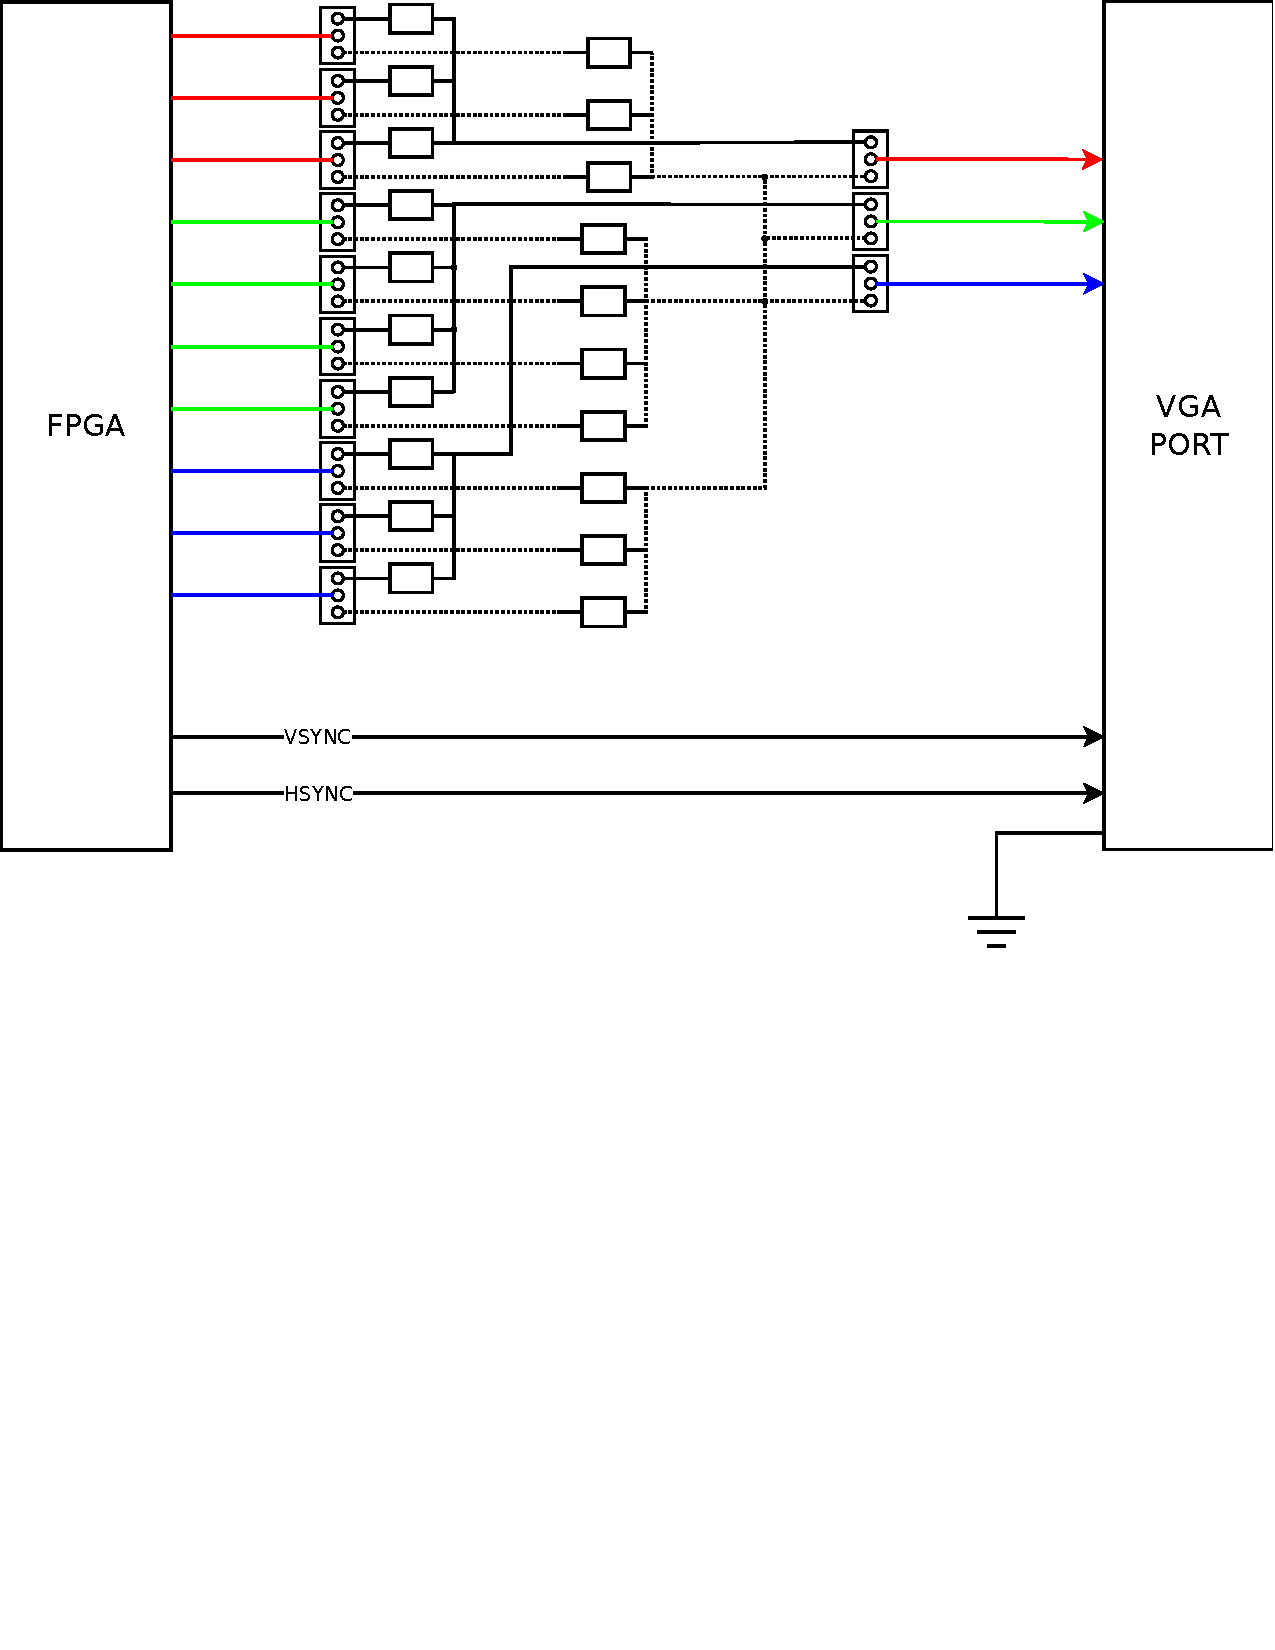
\includegraphics[width=\linewidth,clip,trim=0 11cm 0 0]
                {fig/fpga/vga-circuit.pdf}
\caption[VGA controller]
        {The resistor network of the DAC.}
\label{fig:vga-circuit}
\end{figure}
 When designing the circuit we had to choose between
a black-box\TODO{Call it something else?} \ac{DAC} and making our
own. Preliminary research on the \ac{VGA}-protocol showed that for our purposes
and our fairly low requirements on quality, making the \ac{DAC} with simple
resistors in parallel, with each resistor doubling in resistance for each step
from the most significant bit to the least significant, would be sufficient. We
thought this would be easier to debug, and especially easier to prototype. The
resulting circuit can be seen in figure \ref{fig:vga-circuit}. Since color was a
nice-to-have in case we had time to spare and not at all a priority, we made the
decision to greatly simplify the design by making the switch from greyscale to
color a manual operation of moving a set of jumpers. This way we reduced both
pin-use on the \ac{FPGA} and the complexity of the circuit.
